\documentclass[10pt,t]{beamer}
\usetheme{Heverlee}


%%% QUICK OPTIONS:
% (A) Math font without serifs, enable line below to make math serif:
    %\usefonttheme[onlymath]{serif}

% (B) Re-define primary colour by adjusting the RGB values
    %\definecolor{pblue}	{RGB}{206,125,66}

% (C) Title page graphic (optional) --- this is not for the background image, see \usebackgroundtemplate to change that ---
    %\titlegraphic{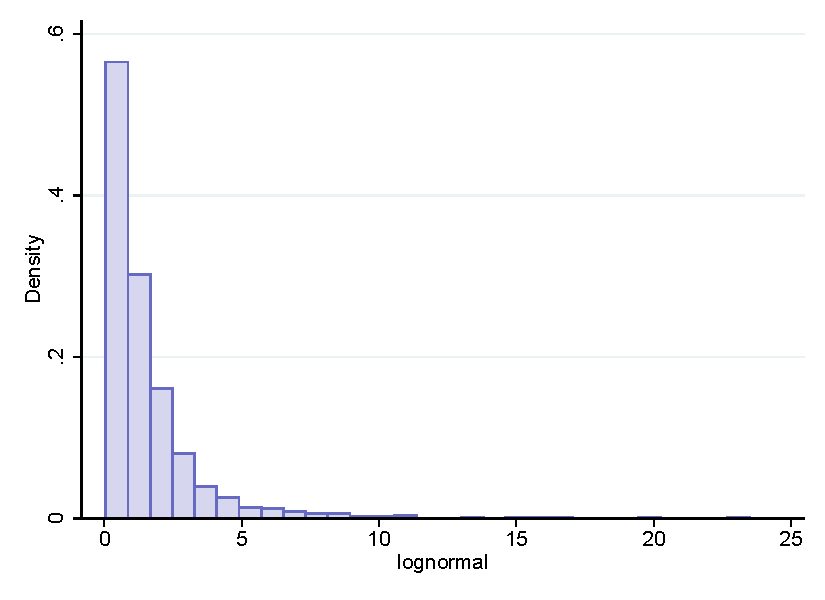
\includegraphics[height=2.7cm]{example_figure.pdf}}

% (D) Add logo to bottom right-corner (optional)
    \logo{
\includegraphics[height=0.7cm]{logo.png}\hspace{12pt}\vspace{-6pt}}      

% (E) Choose one (or none) of these lines to add footline bar on all frames
    %\setbeamertemplate{footline}[infoline]  % author, title, insitute
    %\setbeamertemplate{footline}[navigation] % dots swhowing progress
    %\setbeamertemplate{footline}[navsym] % navigation symbols

% (F) Widescreen 16:9 ratio
    %\usepackage[orientation=landscape,size=custom,width=16,height=9,scale=0.45,debug]{beamerposter} 



%%% TITLE PAGE INFO:
\title[Heverlee \LaTeX\ Beamer theme]{Heverlee Beamer theme}
\subtitle{\textbackslash usetheme\{Heverlee\}}
\author{John Doe}
\institute{Placeholder University}
\date{September 2020}

% Text inside {} is used on the title page. Text inside [] is optional, and is used in footline bar (if [] is omitted then text from {} will be used in both ; if [] is specified but left empty then the footline will not show any text)




 %%
 %%  0. TITLE PAGE and TABLE OF CONTENT
 %%
\begin{document}
% Title page

{
% Change image, or delete this line to remove background image
\usebackgroundtemplate{ \parbox[b][\paperheight][b]{\paperwidth}{\centering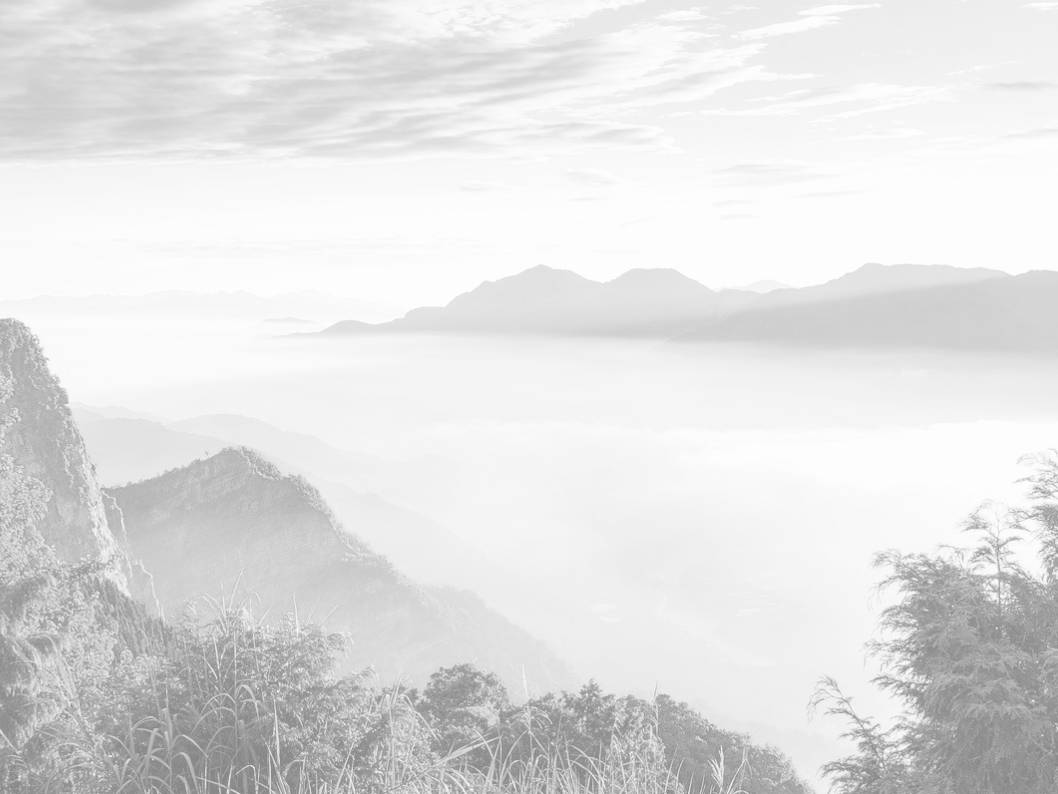
\includegraphics[width=\paperwidth]{Background/bg_alishan.jpg}}} 
 %   abudhabi      cherry      forest      river
 %   alishan       chobe       leuven      sanfancisco
 %   blueprint     columns     library     uyuni
 %   bokeh         flowers     newyork     winter

%\setbeamercolor{background canvas}{bg=lgray}  % make background light gray

\begin{frame}[plain,noframenumbering]
    \titlepage
\end{frame}
}		


% Table of contents slide
\begin{frame}{Outline}
	\vskip 2mm
	\hfill	{\large \parbox{.95\textwidth}{\tableofcontents[hideothersubsections]}}
\end{frame}



 %%
 %%  SECTION 1 - BASIC EXAMPLES
 %%
\section{Basic examples}

\begin{frame}{Color palette}\label{colorpalette}
Recommended, predefined colours
\begin{itemize}
	\item black
	\item \textcolor{pblue}{primary blue} (\texttt{pblue})
	\begin{itemize}
	    \item Can be changed by adding to preamble:
	    \item[ ] \texttt{\textbackslash definecolor\{pblue\}\{RGB\}\{49,130,189\}}
	\end{itemize}
	\item \textcolor{white}{white} $\leftarrow$ white, when background is dark
	\item \textcolor{gray}{50\% gray } for text and \textcolor{lgray}{5\% gray} for background (\texttt{lgray})

	\vspace{5mm}
	\item if necessary use \textcolor{red}{red text color}  
	\item red is also default for \alert{alert text}
\end{itemize}
\end{frame} 



\begin{frame}{Theorems and other blocks}
	\begin{block}{Title of the bloc}
	Text for generic block ...
	\end{block}

\vspace{11pt}
	\begin{exampleblock}{Example block title}
	Text for example block ...
	\end{exampleblock}

\vspace{11pt}
	\begin{alertblock}{Alert block title}
	Text for alert block ...
	\end{alertblock}
\end{frame}




\begin{frame}{Theorems and other blocks}
Theorem environment
	\begin{theorem}
	A theorem is a non-self-evident statement that has been proven to be true.
	\end{theorem}

\vspace{11pt}
Definition environment
	\begin{definition}
	A definition is a statement of the meaning of a term (a word, phrase, or other set of symbols).
	\end{definition}

\vspace{11pt}	
Example environment
	\begin{example}
	Something that serves to illustrate or explain a rule.
	\end{example}
\end{frame}




\begin{frame}{Theorems and other blocks}
Proof environment
	\begin{proof}
	A mathematical proof is an inferential argument for a mathematical statement, showing that the stated assumptions logically guarantee the conclusion.
	\end{proof}
	
\vspace{11pt}	
Corollary environment
	\begin{corollary}
	A corollary is a theorem of less importance which can be readily deduced from a previous, more notable statement.
	\end{corollary}

\end{frame}






\begin{frame}{Buttons}
Standard buttons

	\hyperlink{colorpalette}{\beamergotobutton{Link to frame}}

	\beamerskipbutton{Button with long title and no link}

	\hyperlink{colorpalette}{\beamerreturnbutton{}}

\vspace{11pt}
These buttons can link to any frame, figure, table, theorem, section, or anything else with a defined label.
\end{frame}




 %%
 %%  SECTION 2 - ITEMIZATION
 %%
\section{Itemization and enumeration examples} \label{sec:items}
\begin{frame}{Itemize}
(default)
\begin{itemize}
	\item Itemize style
	\item Itemize style
	\begin{itemize}
		\item Itemize subitem 
		\item Itemize subitem
			\begin{itemize}
				\item Itemize subsubitem
				\item Itemize subsubitem
			\end{itemize}
		\item Itemize subitem	
	\end{itemize}
	\item Itemize style
\end{itemize}
\end{frame}




\begin{frame}{Itemize}
(extra space between items)
\begin{itemize}
	\itemsep 20pt
	\item Itemize style
	\item Itemize style
	\begin{itemize}
		\itemsep 10pt
		\item Itemize subitem
		\item Itemize subitem
		\item Itemize subitem	
	\end{itemize}
	\item Itemize style
\end{itemize}
\end{frame}




\begin{frame}{Enumerate}
(default)
\begin{enumerate}
	\item Enumerate style
	\item Enumerate style
	\begin{enumerate}
		\item Enumerate subitem
		\item Enumerate subitem
		\begin{enumerate}
			\item Enumerate subsubitem
			\item Enumerate subsubitem
		\end{enumerate}
		\item Enumerate subitem
	\end{enumerate}
	\item Enumerate style
\end{enumerate}
\end{frame}




\begin{frame}{Enumerate}
(option I) + pause
\begin{enumerate}[I]
	\item Enumerate style
	\item Enumerate style
	\begin{enumerate}[I]
		\item Enumerate subitem
		\item Enumerate subitem
		\pause
		\begin{enumerate}[I]
			\item Enumerate subsubitem
			\item Enumerate subsubitem
		\end{enumerate}
		\pause
		\item Enumerate subitem
	\end{enumerate}
	\item Enumerate style
\end{enumerate}
\end{frame}




\begin{frame}{Enumerate}
(option i.)
\begin{enumerate}[i.]
	\item Enumerate style
	\item Enumerate style
	\begin{enumerate}[i.]
		\item Enumerate subitem
		\item Enumerate subitem
		\begin{enumerate}[i.]
			\item Enumerate subsubitem
			\item Enumerate subsubitem
		\end{enumerate}
		\item Enumerate subitem
	\end{enumerate}
	\item Enumerate style
\end{enumerate}
\end{frame}




\begin{frame}{Enumerate}
(option A.) + effects
\begin{enumerate}[A.]
	\item<1-5> Enumerate style
	\item<1-5> Enumerate style
	\begin{enumerate}[A.]
		\item<2-5> Enumerate subitem
		\item<3-5> Enumerate subitem
		\begin{enumerate}[A.]
			\item<3-4> Enumerate subsubitem
			\item<3-4> Enumerate subsubitem
		\end{enumerate}
		\item<4-5> Enumerate subitem
	\end{enumerate}
	\item<5> Enumerate style
\end{enumerate}
\end{frame}




\begin{frame}{Enumerate}
(option a + extra space)
\begin{enumerate}[a\enspace]
	\item Enumerate style
	\item Enumerate style
	\begin{enumerate}[a\enspace]
		\item Enumerate subitem
		\item Enumerate subitem
		\begin{enumerate}[a\enspace]
			\item Enumerate subsubitem
			\item Enumerate subsubitem
		\end{enumerate}
		\item Enumerate subitem
	\end{enumerate}
	\item Enumerate style
\end{enumerate}
\end{frame}







 %%
 %%  SECTION 3 - OPTIONS
 %%
\section{Quick options \& customisation}

\begin{frame}[fragile]{(A) Math font}
In preamble of demo.tex there are a few options to easily modify or customise your presentation 

\medskip
Default sans-serif math:
    \begin{itemize}
        \item $ c^2 = a^2+b^2 - 2ab \cos\gamma $
        \item $e^{ \pm i\theta } = \cos \theta \pm i\sin \theta$
    \end{itemize}

\medskip
To change to serif math everywhere

    \begin{itemize}
        \item $ \mathnormal{c^\mathrm{2} = a^\mathrm{2}+b^\mathrm{2} - \mathrm{2}ab \cos\gamma} $
        \item $\mathnormal{e^{ \pm i\theta } = \cos \theta \pm i\sin \theta}$
    \end{itemize}
\medskip
\verb+  \usefonttheme[onlymath]{serif}+

\end{frame}




\begin{frame}[fragile]{(B) Change primary colour}
    \begin{itemize}
        \item Default color for frame titles, itemization and other elements is \textcolor{pblue}{blue}
        \item You can redefine primary color, to e.g. orange, by changing RGB values:
    \end{itemize}

\medskip
\verb+\definecolor{pblue}{RGB}{+{\color{red}\verb+206,125,66+}\verb+}+
\end{frame}


\begin{frame}[fragile]{(C) First page foreground image}
    \begin{itemize}
        \item Add additional small foreground image on the title page
        \item Add in preamble:
    \end{itemize}

\vspace{12pt}
\begin{verbatim}
\titlegraphic{\includegraphics[height=3cm]{myimage.png}}
\end{verbatim}

\medskip
\centering Not that this not for the background image. Go to: \hyperlink{background_image}{\beamergotobutton{First page background}}

\end{frame}



\begin{frame}[fragile]{(D) Footline logo}
\begin{itemize}
    \item Add your logo in bottom right corner
    \item Command \verb+\logo+ can be removed, and no logo will be shown
\end{itemize}

\vspace{12pt}
\begin{verbatim}
\logo{
\includegraphics[height=0.7cm]{logo.png}\hspace{12pt}
    \vspace{-6pt}}
\end{verbatim}




\end{frame}




\begin{frame}[fragile]{(E) Footline information bar}
\begin{itemize}
    \item Add information on bottom of every frame
    \item Four options:
    \begin{itemize}
        \item \verb+infoline+ ~:~ Text line with author, titile and institute
        \item \verb+navigation+  ~:~ Dots by frame and section showing progress
        \item \verb+navsym+  ~:~ Navigation symbols
        \item Nothing (delete/disable all)
    \end{itemize}
    \smallskip
    \item Options cannot be combined
    \item Can be combined with logo
    
\end{itemize}

\medskip
\verb+\setbeamertemplate{footline}[+{\color{red}\verb+infoline+}\verb+]+
\end{frame}






\begin{frame}[fragile]{(F) Widescreen}
	Default screen ration is 4:3.  Load the following package in the preamble to make all frames wider to 16:9 ratio:
	
	\begin{verbatim}
	\usepackage[orientation=landscape,size=custom,
	width=16,height=9,scale=0.45,debug]{beamerposter} 
	\end{verbatim}
	
	Title page or other frames should not get (too) distorted because of it. 
\end{frame}

















 %%
 %%  SECTION 4 - GALLERY
 %%
\section{Title page background templates gallery}
\begin{frame}[fragile]{First page background}\label{background_image}
    \begin{itemize}
        \item Easily change first page background image with a selection of templates, or any photo you want (change filename \textcolor{red}{in red})
        \item All included images are based on photos that free for commercial and non-commercial use. Attribution is not required.
        \item Background image can be removed (delete the entire line)
    \end{itemize}
    
  \vspace{6pt}  
\verb+{+ \\

\verb+\usebackgroundtemplate{+{\color{gray} \verb+\parbox[b][\paperheight]+

    \verb+[b]{\paperwidth}{\centering+
\color{black}\verb+\includegraphics+
\color{gray} \verb+[width=\paperwidth]+\color{black}\verb+{Background/+\color{red} \verb+bg_alishan.jpg+\color{black}\verb+}+\color{gray} \verb+}+\color{black}\verb+}+ 
}

\smallskip
\verb+\begin{frame}[plain,noframenumbering]+ \\
\verb+  \titlepage+ \\
\verb+\end{frame}+ \\
\verb+}+

\vspace{12pt}  
\footnotesize{Part in \textcolor{gray}{gray} is is not always necessary. It ensures the images of various sizes will fit and are aligned.}
\end{frame}






{
\usebackgroundtemplate{ \parbox[b][\paperheight][b]{\paperwidth}{\centering
\includegraphics[width=\paperwidth]{Background/bg_abudhabi.jpg}}} 
\begin{frame}[plain,noframenumbering]
    \titlepage
\end{frame}
}

{
\usebackgroundtemplate{ \parbox[b][\paperheight][b]{\paperwidth}{\centering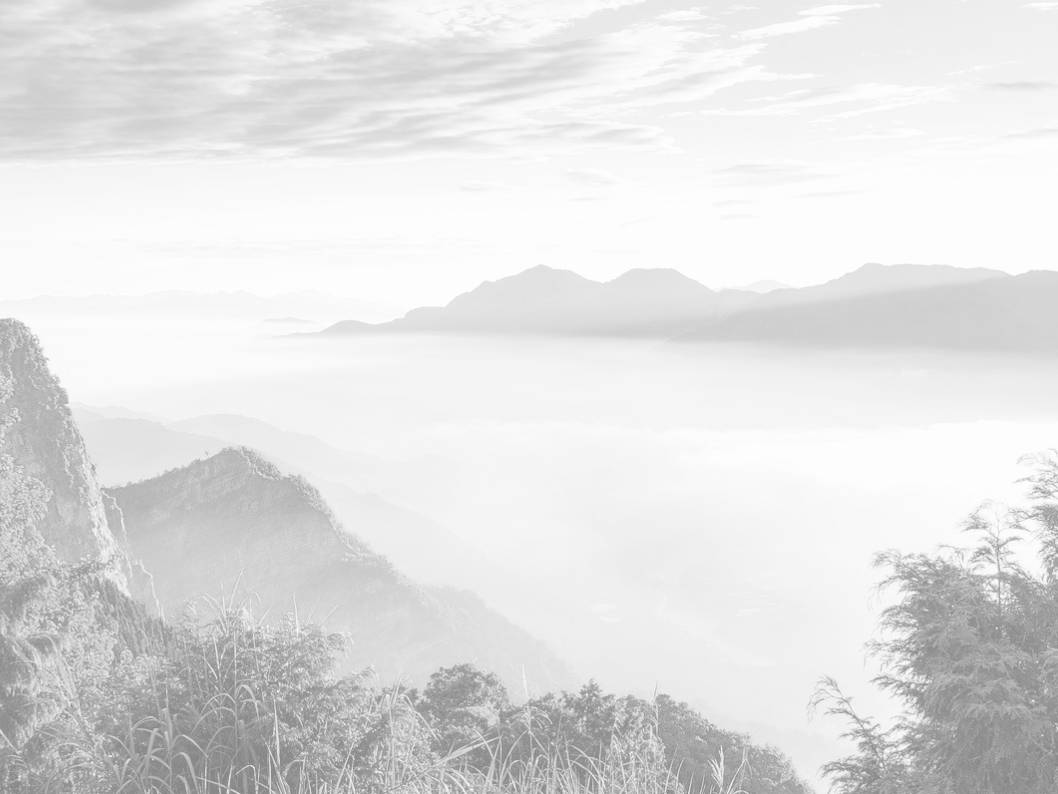
\includegraphics[width=\paperwidth]{Background/bg_alishan.jpg}}} 
\begin{frame}[plain,noframenumbering]
    \titlepage
\end{frame}
}

{
\usebackgroundtemplate{ \parbox[b][\paperheight][b]{\paperwidth}{\centering
\includegraphics[width=\paperwidth]{Background/bg_blueprint.jpg}}} 
\begin{frame}[plain,noframenumbering]
    \titlepage
\end{frame}
}


{
\usebackgroundtemplate{ \parbox[b][\paperheight][b]{\paperwidth}{\centering
\includegraphics[width=\paperwidth]{Background/bg_bokeh.jpg}}} 
\begin{frame}[plain,noframenumbering]
    \titlepage
\end{frame}
}


{
\usebackgroundtemplate{ \parbox[b][\paperheight][b]{\paperwidth}{\centering
\includegraphics[width=\paperwidth]{Background/bg_cherry.jpg}}} 
\begin{frame}[plain,noframenumbering]
    \titlepage
\end{frame}
}


{
\usebackgroundtemplate{ \parbox[b][\paperheight][b]{\paperwidth}{\centering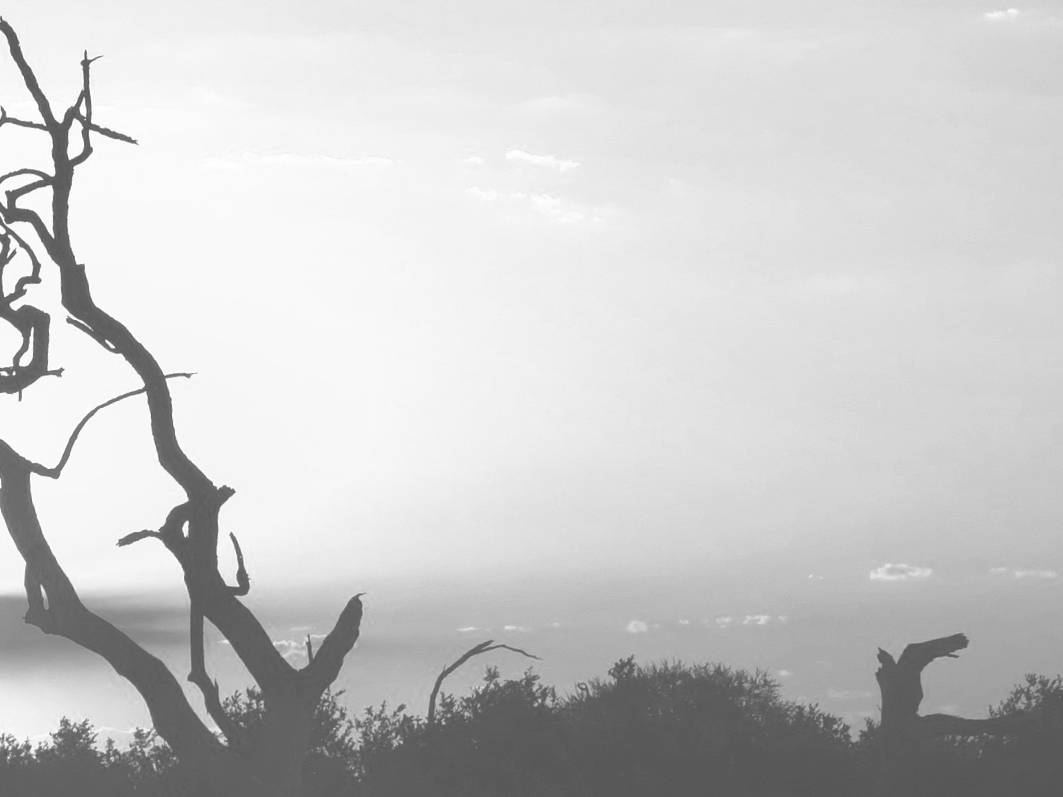
\includegraphics[width=\paperwidth]{Background/bg_chobe.jpg}}} 
\begin{frame}[plain,noframenumbering]
    \titlepage
\end{frame}
}


{
\usebackgroundtemplate{ \parbox[b][\paperheight][b]{\paperwidth}{\centering
\includegraphics[width=\paperwidth]{Background/bg_columns.jpg}}} 
\begin{frame}[plain,noframenumbering]
    \titlepage
\end{frame}
}


{
\usebackgroundtemplate{ \parbox[b][\paperheight][b]{\paperwidth}{\centering
\includegraphics[width=\paperwidth]{Background/bg_flowers.jpg}}} 
\begin{frame}[plain,noframenumbering]
    \titlepage
\end{frame}
}


{
\usebackgroundtemplate{ \parbox[b][\paperheight][b]{\paperwidth}{\centering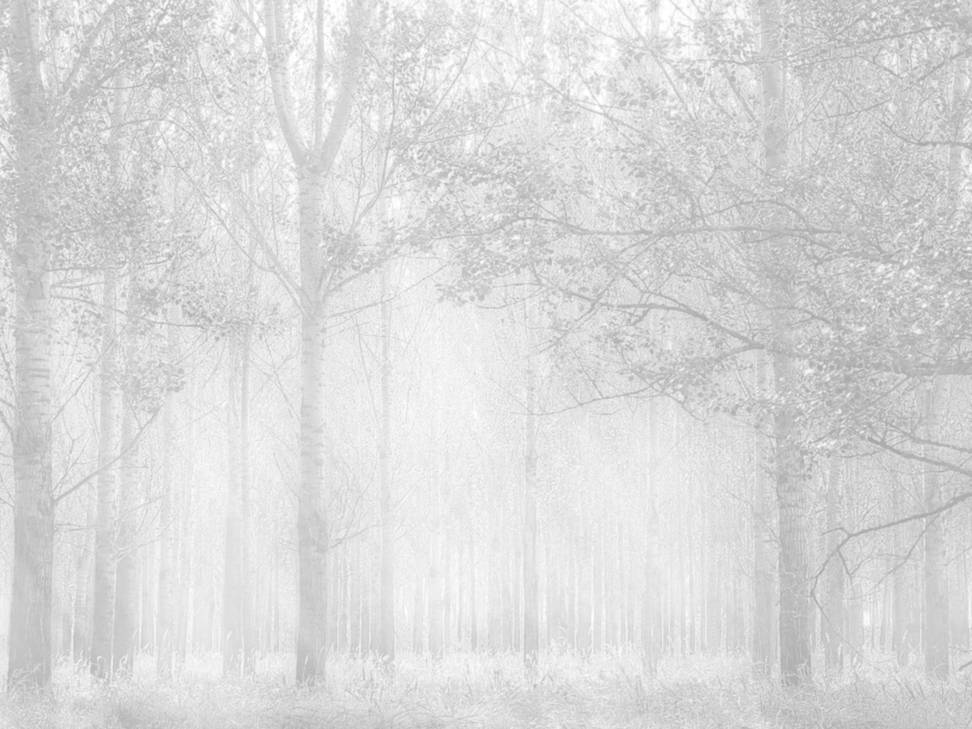
\includegraphics[width=\paperwidth]{Background/bg_forest.jpg}}} 
\begin{frame}[plain,noframenumbering]
    \titlepage
\end{frame}
}



{
\usebackgroundtemplate{ \parbox[b][\paperheight][b]{\paperwidth}{\centering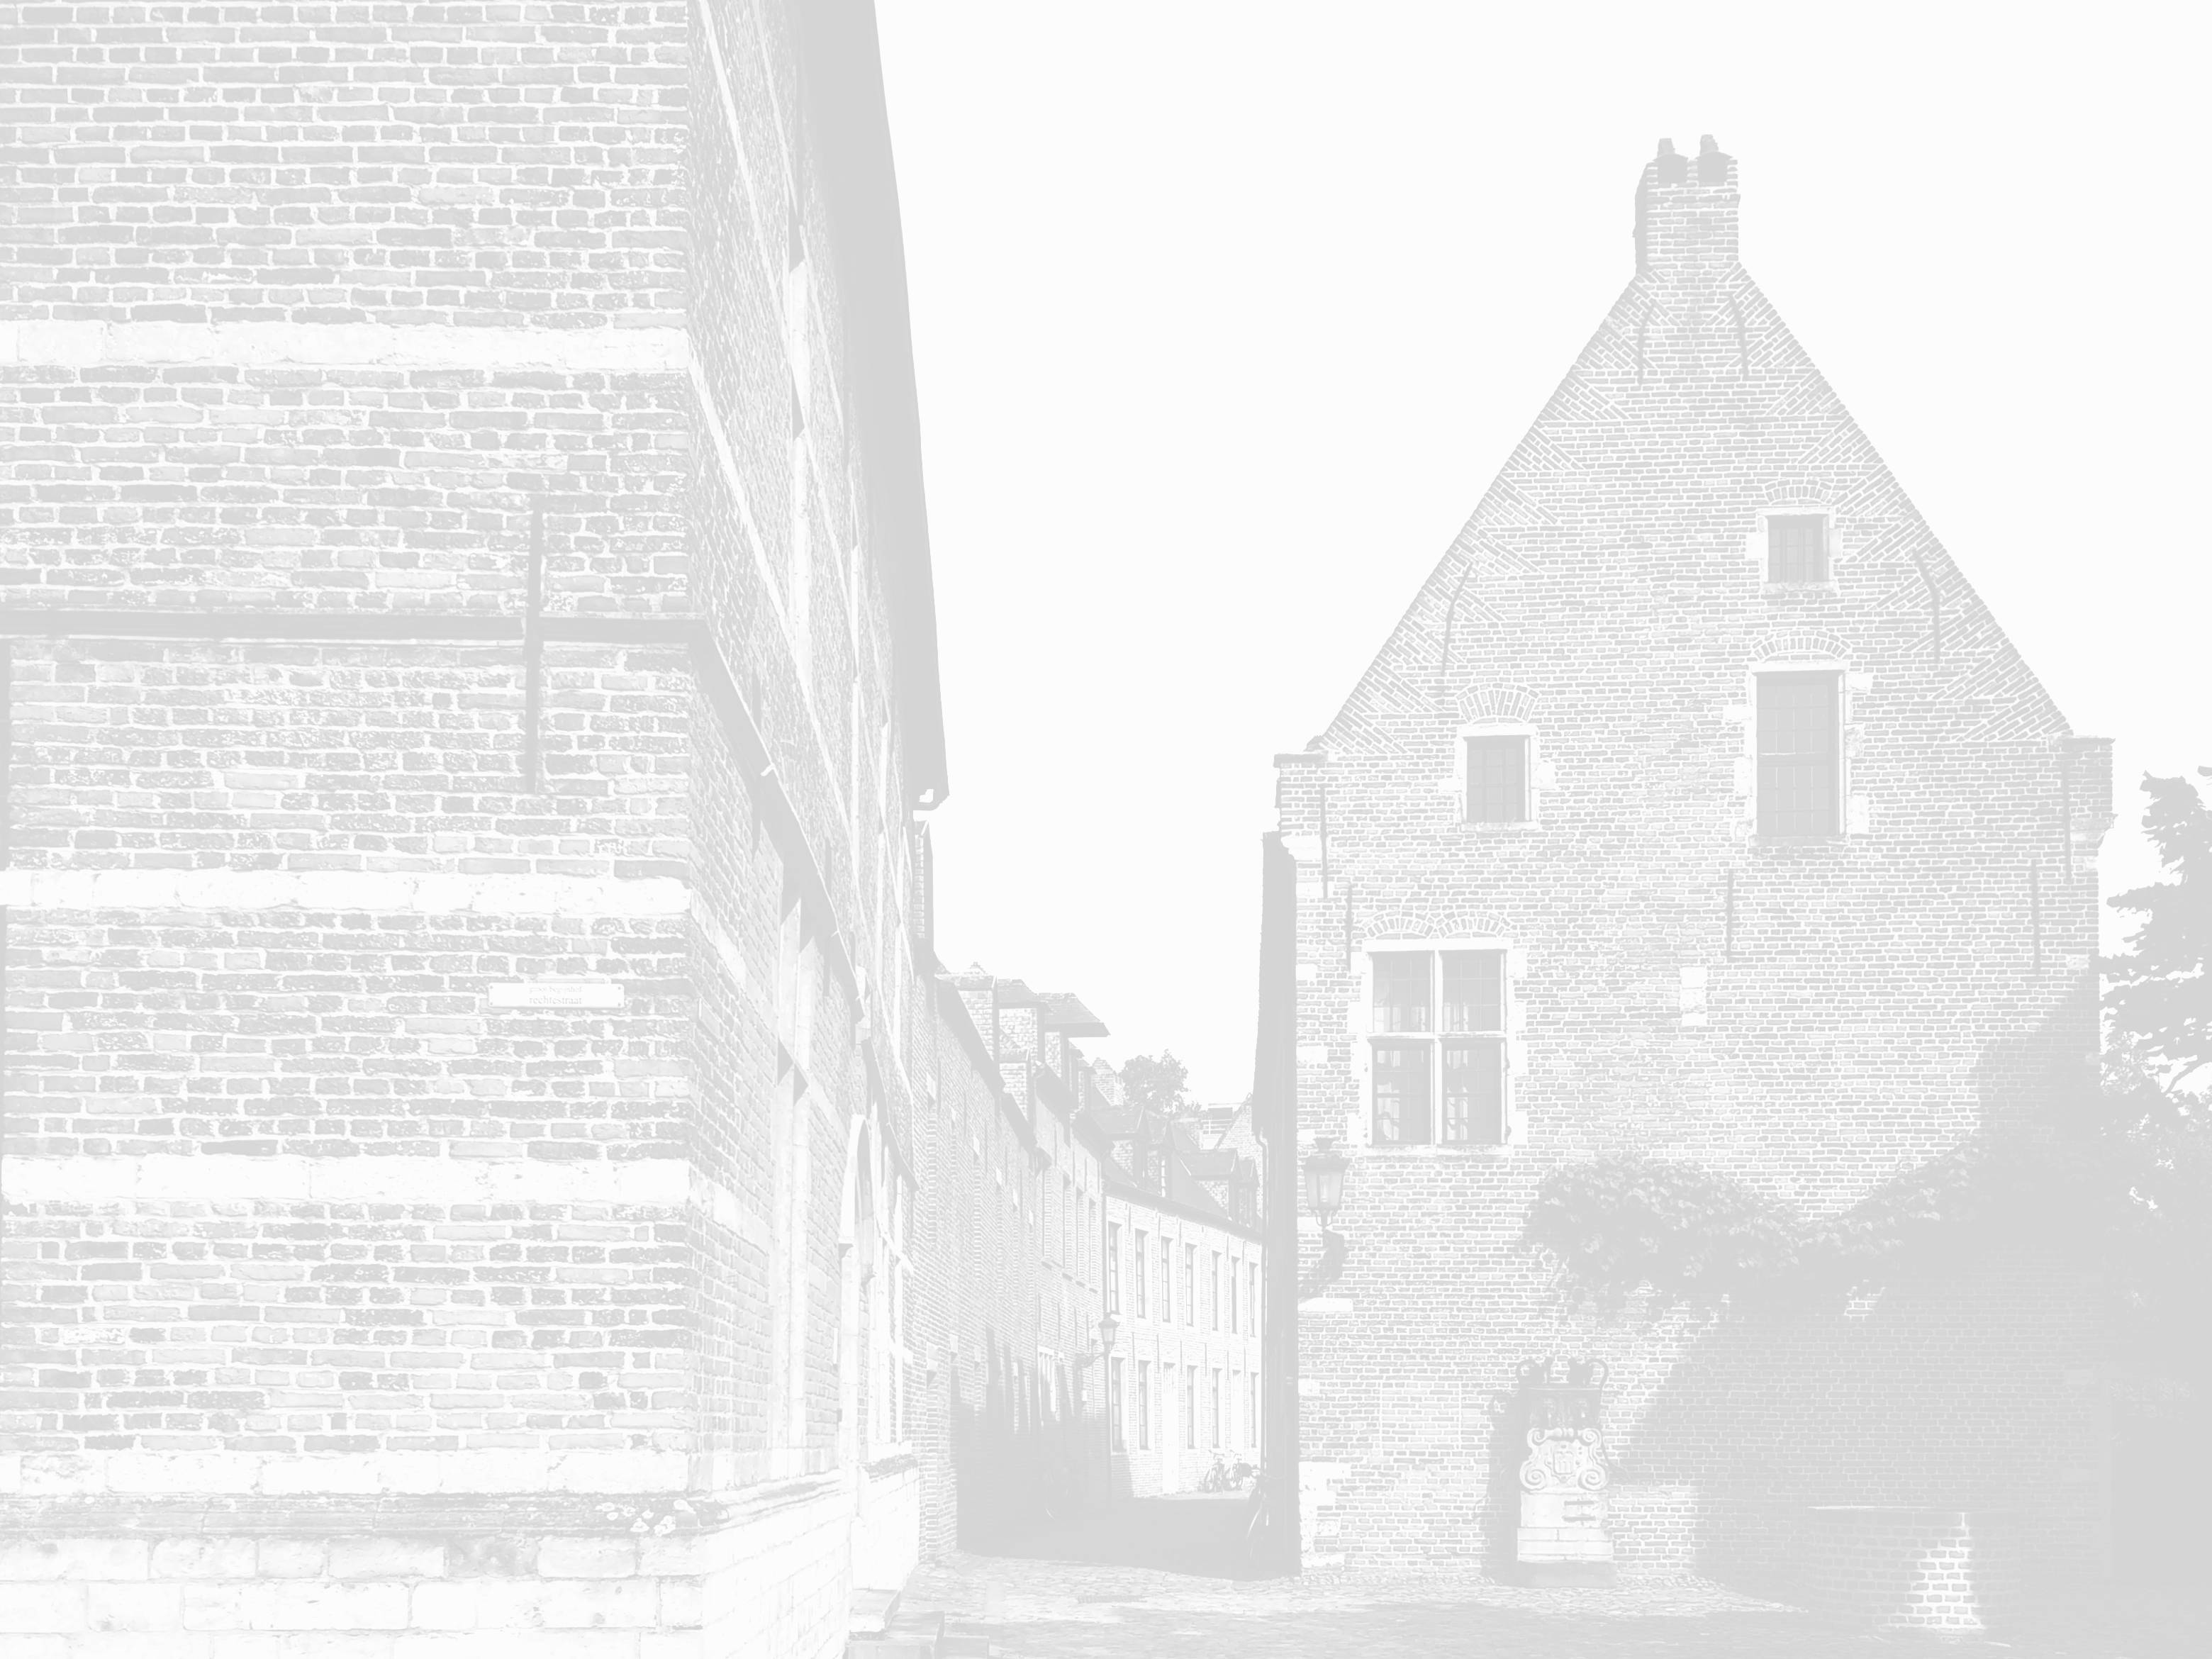
\includegraphics[width=\paperwidth]{Background/bg_leuven.jpg}}} 
\begin{frame}[plain,noframenumbering]
    \titlepage
\end{frame}
}

{
\usebackgroundtemplate{ \parbox[b][\paperheight][b]{\paperwidth}{\centering
\includegraphics[width=\paperwidth]{Background/bg_library.jpg}}} 
\begin{frame}[plain,noframenumbering]
    \titlepage
\end{frame}
}

{
\usebackgroundtemplate{ \parbox[b][\paperheight][b]{\paperwidth}{\centering
\includegraphics[width=\paperwidth]{Background/bg_newyork.jpg}}} 
\begin{frame}[plain,noframenumbering]
    \titlepage
\end{frame}
}


{
\usebackgroundtemplate{ \parbox[b][\paperheight][b]{\paperwidth}{\centering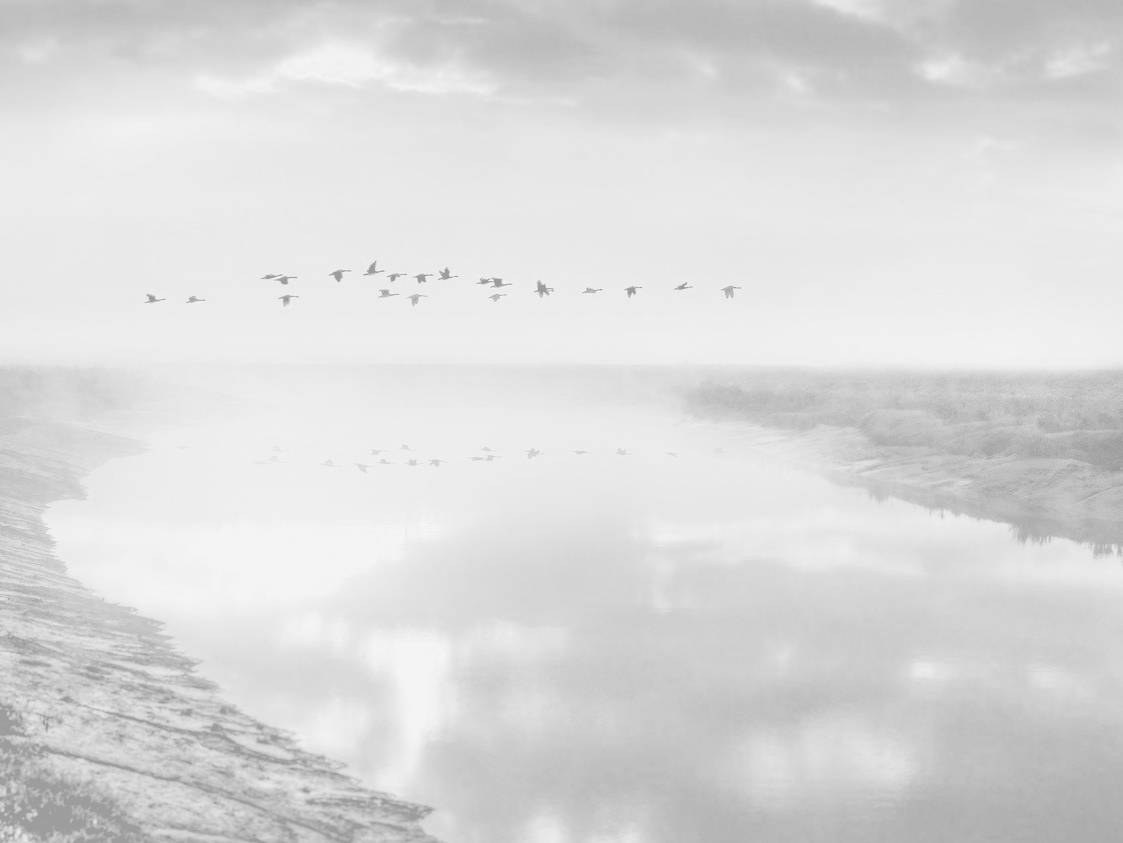
\includegraphics[width=\paperwidth]{Background/bg_river.jpg}}} 
\begin{frame}[plain,noframenumbering]
    \titlepage
\end{frame}
}

{
\usebackgroundtemplate{ \parbox[b][\paperheight][b]{\paperwidth}{\centering
\includegraphics[width=\paperwidth]{Background/bg_sanfrancisco.jpg}}} 
\begin{frame}[plain,noframenumbering]
    \titlepage
\end{frame}
}


{
\usebackgroundtemplate{ \parbox[b][\paperheight][b]{\paperwidth}{\centering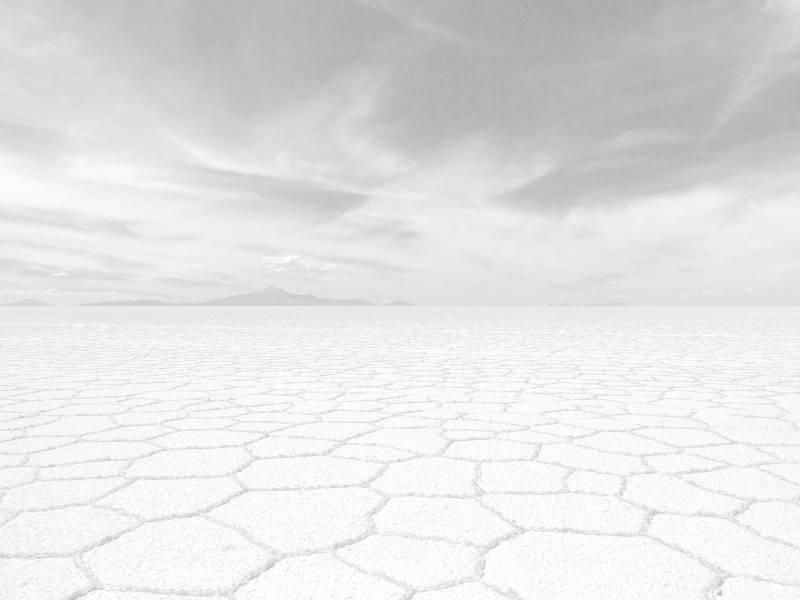
\includegraphics[width=\paperwidth]{Background/bg_uyuni.jpg}}} 
\begin{frame}[plain,noframenumbering]
    \titlepage
\end{frame}
}



{
\usebackgroundtemplate{ \parbox[b][\paperheight][b]{\paperwidth}{\centering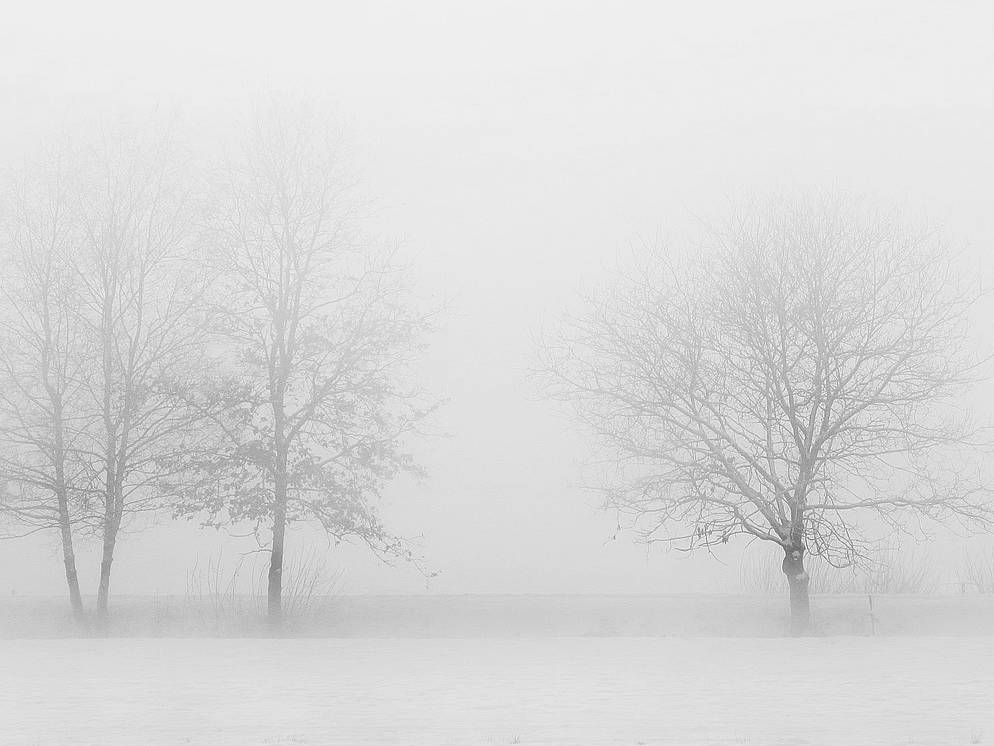
\includegraphics[width=\paperwidth]{Background/bg_winter.jpg}}} 
\begin{frame}[plain,noframenumbering]
    \titlepage
\end{frame}
}


{

\setbeamercolor{background canvas}{bg=gray}
\begin{frame}[c,plain]{}
    \centering
    \textcolor{white}{Thank you}
\end{frame}

}














\end{document}
